
\documentclass[ fontsize=11pt]{scrartcl} % A4 paper and 11pt font size

%%%%%%%%%%%%%%%%%%%%%%%%%%%%%%%%%%%%%%%%%%%%%%%%%%%%%%%%%%%%
%PICTURES
%%%%%%%%%%%%%%%%%%%%%%%%%%%%%%%%%%%%%%%%%%%%%%%%%%%%%%%%%%%%

\usepackage[]{graphicx} % for inserting figure, graphics,...
%\usepackage{subfigure} % conflict with subcaption
\usepackage{subcaption}

%%%%%%%%%%%%%%%%%%%%%%%%%%%%%%%%%%%%%%%%%%%%%%%%%%%%%%%%%%%%
%MARGINS & LAYOUT
%%%%%%%%%%%%%%%%%%%%%%%%%%%%%%%%%%%%%%%%%%%%%%%%%%%%%%%%%%%%
\usepackage{makeidx}

\usepackage{vmargin}
\setpapersize{A4}
\setmarginsrb{20mm}{5mm}{20mm}{15mm}
             {0mm}{7mm}{0mm}{10mm}
\setlength\parindent{0pt} % Removes all indentation from paragraphs - comment this line for an assignment with lots of text
\usepackage{array,makecell} %centering and manipulating cells in tables
%%%%%%%%%%%%%%%%%%%%%%%%%%%%%%%%%%%%%%%%%%%%%%%%%%%%%%%%%%%%
%LANGUAGE & FONT
%%%%%%%%%%%%%%%%%%%%%%%%%%%%%%%%%%%%%%%%%%%%%%%%%%%%%%%%%%%%

\usepackage[utf8]{inputenc} %& parole accentate (italiane!)

\usepackage{fourier} % Use the Adobe Utopia font for the document - comment this line to return to the LaTeX default
\usepackage[british]{babel} % English language/hyphenation

\usepackage{lipsum} % Used for inserting dummy 'Lorem ipsum' text into the template

\usepackage[T1]{fontenc} % Use 8-bit encoding that has 256 glyphs

\usepackage{fancyhdr} % Custom headers and footers
\pagestyle{fancyplain} % Makes all pages in the document conform to the custom headers and footers
\fancyhead{} % No page header - if you want one, create it in the same way as the footers below
\fancyfoot[L]{} % Empty left footer
\fancyfoot[C]{} % Empty center footer
\fancyfoot[R]{\thepage} % Page numbering for right footer
\renewcommand{\headrulewidth}{0pt} % Remove header underlines
\renewcommand{\footrulewidth}{0pt} % Remove footer underlines
\setlength{\headheight}{10.6pt} % Customize the height of the header

%%%%%%%%%%%%%%%%%%%%%%%%%%%%%%%%%%%%%%%%%%%%%%%%%%%%%%%%%%%%%%%
%MATH & PHYSICS
%%%%%%%%%%%%%%%%%%%%%%%%%%%%%%%%%%%%%%%%%%%%%%%%%%%%%%%%%%%%%%%
\usepackage{amsmath,amsfonts,amsthm} % Math packages
\usepackage{physics} %per scrivere veloce derivate parziali, ecc...
\usepackage{amssymb} %for gather and aligned type equation (multiline)
\usepackage{gensymb} %for degree symbol
\numberwithin{equation}{section} % Number equations within sections (i.e. 1.1, 1.2, 2.1, 2.2 instead of 1, 2, 3, 4)
\numberwithin{figure}{section} % Number figures within sections (i.e. 1.1, 1.2, 2.1, 2.2 instead of 1, 2, 3, 4)
\numberwithin{table}{section} % Number tables within sections (i.e. 1.1, 1.2, 2.1, 2.2 instead of 1, 2, 3, 4)
\usepackage{empheq} % for equation in box
\newcommand*\widefbox[1]{\fbox{\hspace{2em}#1\hspace{2em}}} %forboxes
\usepackage{enumitem} % for description (list of symbols chapter)
\usepackage{siunitx}

\newtheorem{myprop}{Property}
\newtheorem{myproof}{Proof}
\newtheorem{example}{Example}



%\usepackage{sectsty} % Allows customizing section commands
%\allsectionsfont{\centering \normalfont\scshape} % Make all sections centered, the default font and small caps


%%%%%%%%%%%%%%%%%%%%%%%%%%%%%%%%%%%%%%%%%%%%%%%%%%%%%%%%%%%%%%%%%%%%%%%%%%%%%%
%	TITLE SECTION
%%%%%%%%%%%%%%%%%%%%%%%%%%%%%%%%%%%%%%%%%%%%%%%%%%%%%%%%%%%%%%%%%%%%%%%%%%%%%%

\newcommand{\horrule}[1]{\rule{\linewidth}{#1}} % Create horizontal rule command with 1 argument of height

\title{	
\normalfont \normalsize 
\textsc{Istituto Nazionale di RIcerca Metrologica } \\ [10pt]
%\textsc{} \\ [10pt] % university, school and/or department name(s)
\horrule{0.7pt} \\[0.4cm] % Thin top horizontal rule
\huge Polarization-insensitive phase recovery in optical fiber link for frequency metrology \\ % The assignment title
\horrule{3pt} \\[0.5cm] % Thick bottom horizontal rule
}

\author{Stefano Paracchino} % Your name

\date{Update: October 2018} % Today's date or a custom date



%%%%%%%%%%%%%%%%%%%%%%%%%%%%%%%%%%%%%%%%%%%%%%%%%%%%%%%%%%%%%%%%%%%%%%%%%%%%%%%%
%%%%%%%%%%%%%%%%%%%%%%%%%%%%%%%%%%%%%%%%%%%%%%%%%%%%%%%%%%%%%%%%%%%%%%%%%%%%%%%%%
%%%%%%%%%%%%%%%%%%%%%%%%%%%%%%%%%%%%%%%%%%%%%%%%%%%%%%%%%%%%%%%%%%%%%%%%%%%%%%%%%%
\begin{document}

\maketitle
\tableofcontents 
\pagebreak

\section{Noise sensitivity of the algorithm}
\subsection{Theoretical background}\label{back}

In order to perform simulations with a good reliability, few fundamental sources of random processes must be taken into account:

\begin{itemize}
\item \textsl{intrinsic noise:} this is actually the metrological information we want to reveal. A clock stability as well as the optical link performance is measured in terms of noise power spectral density. In particular, considering that these measurements are based on the phase difference between two oscillators, we are interested in the phase noise power spectral density (PSD) $S_{\phi}(f)$ $\left(\frac{\text{rad}^2}{\text{Hz}}\right)$.
This quantity is usually modeled using a power-law function $S_{\phi}(f)=b_0 \, f^{0} + b_1 \, f^{-1}+ b_2 \, f^{-2}+ b_3 \, f^{-3}+...$ which corresponds, in the typical log-log plot, to a sum of lines with different slope.\\
Recalling that $S_{\phi}(f)$ is intended to be one-side PSD \footnote{The PSD of a real function is an even function. Furthermore the one-side PSD is what is displayed by a spectrum analyzer instrument.}, namely:
\begin{equation}
S(f)=\frac{2}{T}\left|\hat{X}(f)\right|^2
\end{equation}
where $T$ is the measurement time and $\hat{X}(f)$ is the Fourier Transform in the frequency domain $f$. \\
Moving to the digital domain, the one-side PSD becomes:
\begin{equation}
S(\mathtt{F})=\frac{2}{N\cdot f_s}\left|\hat{X}(F)\right|^2
\end{equation}
where $N$ is the number of samples and $f_s$ is the sampling frequency, while $F$ is the digital (discrete) frequency.\\
However for a preliminary analysis, a simpler model $S_{\phi}(f)=b_0 \, f^{0} + b_2 \, f^{-2}$ will be considered, whose terms are called respectively \textit{white noise}  and \textit{random walk (noise)}.  In this case, only two meaningful quantities must be known to fully describe the function: the $b_0$ factor for the white noise and the $b_2 \cdot(1)^{-2}=b_2$  product \footnote{$b_2$ unit of measurement is \SI{}{\radian\squared\hertz}} i.e. the noise value at $f=1$ for the random walk term.

\item \textsl{detection noise:} this is due to the opto-electronic read-out system. In spite of the several phenomena involved for a complete noise description (shot noise, flickering,...) we choose  for a preliminary analysis a simplified model as above. This takes  into account the only contribution of the white noise. In particular, the four channels are considered uncorrelated i.e. each one is characterized by a single white noise random process. 

\item \textsl{quantization noise:} this phenomenon arises from the ADC process. A correspondence between the time and frequency domains is quite complex to be derived, but the frequency spectrum can be assumed flat (i.e. quantization noise becomes white) for the whiteness condition \footnote{Eq (20.54) of http://oldweb.mit.bme.hu/books/quantization/spectrum.pdf}:
\begin{equation}
f_s<9.2 \frac{\sigma_x}{q}BW=9.2\frac{1}{\sqrt{12}}BW\approx 2.7BW
\end{equation}
The condition can thus be satisfied for an observed signal with frequencies components which extend up to near the nyquist frequency.

\end{itemize}

In Digital Signal Process, random processes such as white noise and random walk are modeled with a sequence of data arising from random data generation. In the former case every value of the sequence is obtained with the formula $A_{\text{wn}} \cdot \mathcal{N}(0,1) $ where $\mathcal{N}(0,1) $ is a value randomly extracted from a Normal Distribution with zero mean and unitary variance while the values of a random walk sequence are $A_{\text{rw}} \cdot \mathcal{C}(\mathcal{N}(0,1) )$ where  $\mathcal{C}(\mathcal{N}(0,1) )$ is the cumulative sum of the white noise n-length sequence up to the considered n-th value.
The magnitudes of the amplitudes $A_{\text{wn}}$ and $A_{\text{rw}}$ are determined respectively by the chosen values for $b_0$ and $b_2$ as described in Tab.(\ref{pow-amp}).


\begin{table}[htb]
\centering
\begin{tabular}{cccll}
\cline{1-4}
\multicolumn{1}{|c|}{}                                                      & \multicolumn{1}{c|}{Amplitude \SI{}{(\radian)}} & \multicolumn{1}{c|}{PSD  \SI{}{(\radian\squared\per\hertz)}} & \multicolumn{1}{c|}{Applied to:} &  \\ \cline{1-4}
\multicolumn{1}{|c|}{\begin{tabular}[c]{@{}c@{}}random\\ walk\end{tabular}} & \multicolumn{1}{c|}{$A_{\text{wn}}=\sqrt{\frac{2 \pi^2 b_2}{f_s}}$ }          & \multicolumn{1}{c|}{$b_2\cdot(1)^{-2}=b_2$  }       & \multicolumn{1}{c|}{Simul. params} &  \\ \cline{1-4}
\multicolumn{1}{|c|}{\begin{tabular}[c]{@{}c@{}}white\\ noise\end{tabular}} & \multicolumn{1}{c|}{$A_{\text{rn}}=\sqrt{\frac{b_0 f_s}{2}}$ }          & \multicolumn{1}{c|}{$b_0$}      & \multicolumn{1}{c|}{Simul. electr. channels} &  \\ \cline{1-4}
\multicolumn{1}{|c|}{\begin{tabular}[c]{@{}c@{}}quant\\ noise\end{tabular}} & \multicolumn{1}{c|}{}          & \multicolumn{1}{c|}{$b_q$ }      & \multicolumn{1}{c|}{Simul. electr. channels} &  \\ \cline{1-4}
\multicolumn{1}{l}{}                                                        & \multicolumn{1}{l}{}           & \multicolumn{1}{l}{}       &  & 
\end{tabular}
\caption{Amplitude-PSD relation for random processes}
\label{pow-amp}
\end{table}
\pagebreak

The starting point for our noise sensitivity analysis is the choice of proper values for $b_0$ and $b_2$.\\ Fig(\ref{psd_long}) shows a typical optical fiber link phase noise spectrum for an installed long distance optical link  ($\approx 10^2$ \SI{}{\kilo\meter}) while Fig(\ref{psd_short}) illustrates the spectrum obtained via the recovery algorithm in a lab setup, where the total length is limited for testing reasons to just  few meters.\\
Both show the same "$f^{-2}$ shape" for all the low frequency range and the "flat shape" for the higher one.
Furthermore they share the same ratio between the phase noise at 1 Hz ($b_2$ value) and the value of the white noise plateau which is around $10^{7}-10^{8}$.
We will therefore model the noise sources of Tab(\ref{pow-amp}) assuming the above power ratio, and we will chose the absolute value for $b_2$ from Fig(\ref{psd_short}). However the spectrum in Fig(\ref{psd_short}) does not represents a "pure" random walk spectrum in fact the phase signal is also formed with an important contribute of low a frequency component (<1 Hz). This component overlaps in the frequency domain the random walk spectrum. Therefore a more reliable value for $b_2$ to be adopted in the simulations is around two order of magnitude less than the one obtained in Fig(\ref{psd_short}): 1 \SI{}{\radian\squared\per\hertz} $\rightarrow$ 0.01 \SI{}{\radian\squared\per\hertz}. (Furthermore we cannot build a random walk process from the plot of Fig(\ref{psd_long}) if we do not know the sampling frequency)

\begin{figure}[hbtp]
\centering
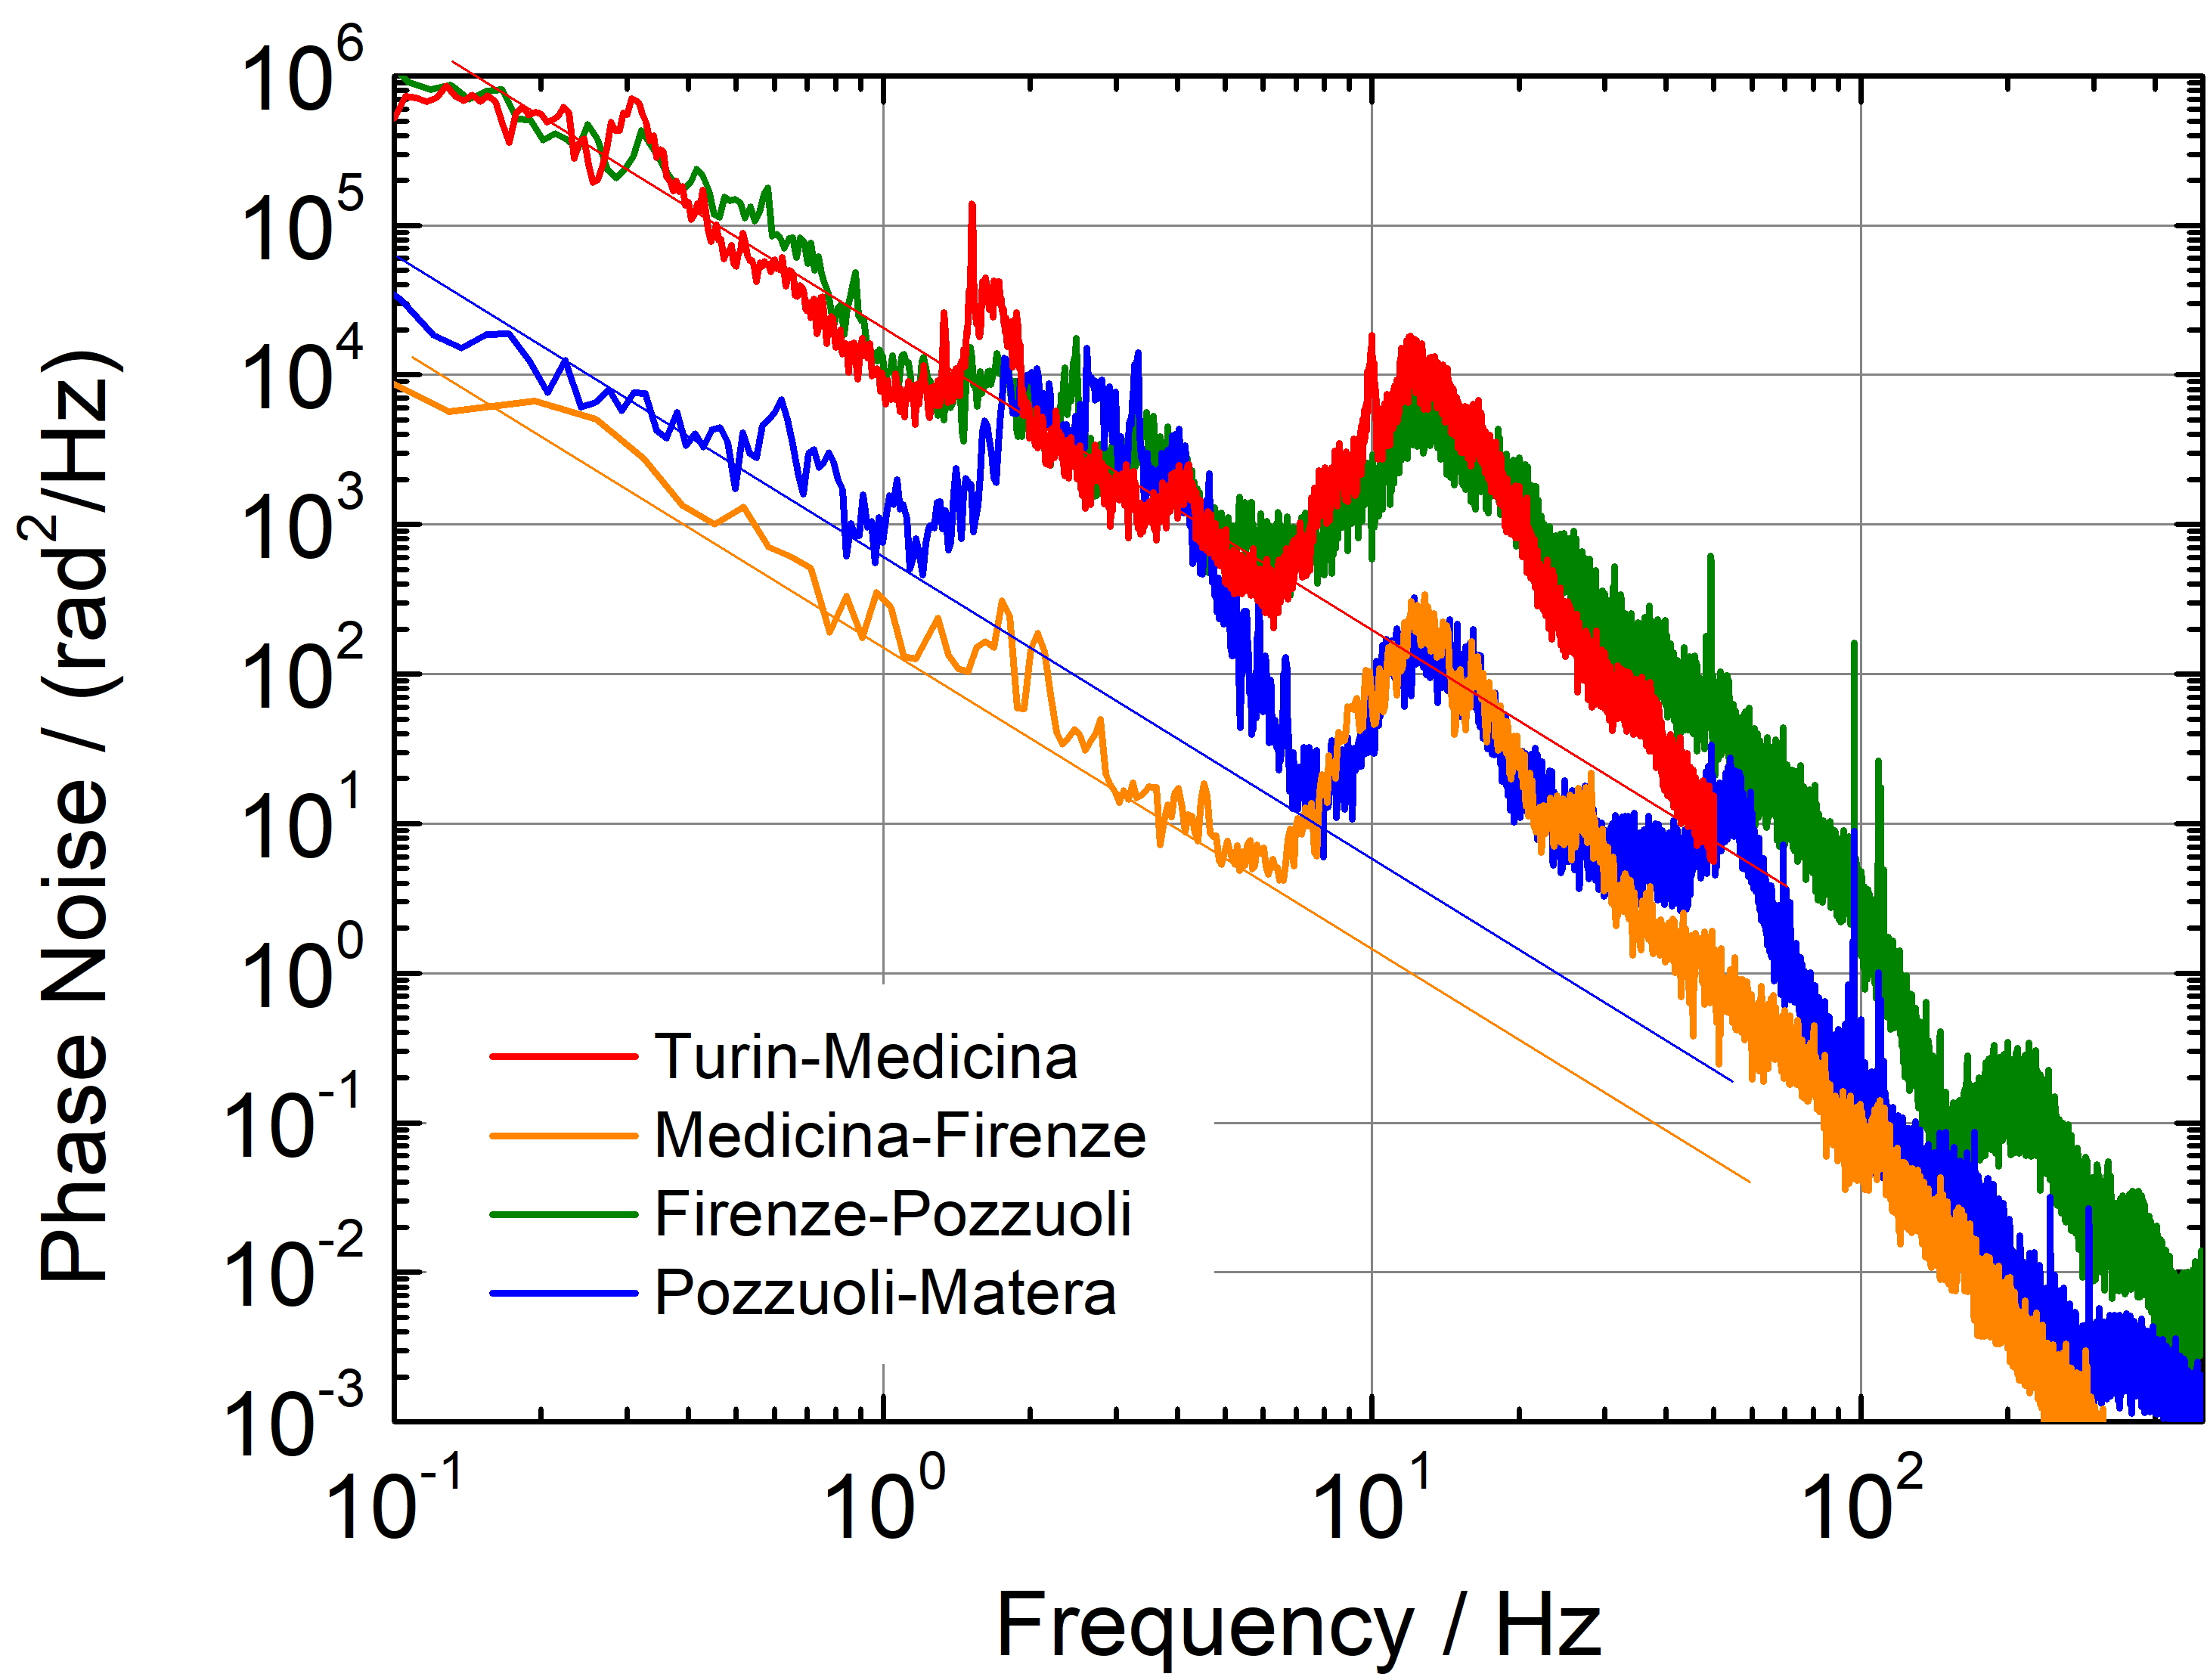
\includegraphics[scale=0.45]{immagini_noise/noise_long.png}
\caption{Phase PSD for a long distance link in a real frequency dissemination system}
\label{psd_long}
\end{figure}

\begin{figure}[hbtp]
\centering
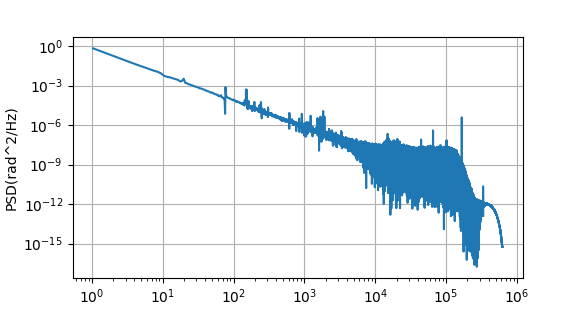
\includegraphics[scale=0.75]{immagini_noise/noise_short.png}
\caption{Phase PSD for a long short link in lab environment. (downsampling=2, lowfilter=100kHz)}
\label{psd_short}
\end{figure}

\pagebreak

\subsection{Step 1: Random Walk affecting the parameters}

As stated in the previous chapter, we add a random walk noise on all the three parameters $\delta$,$\theta$,$\phi$. Fig.(\ref{randwalk_par}) shows the result for a simple case where the optical fiber parameters ($\delta$,$\theta$) are simply set to sinusoidal functions while $\phi$ is set to zero (therefore, it becomes a "pure" random walk signal). The corresponding PSD spectrum of $\phi$ is shown in Fig.(\ref{PSD_phi}).
\begin{center}
\begin{figure}[hbtp]
 \makebox[\textwidth][c]{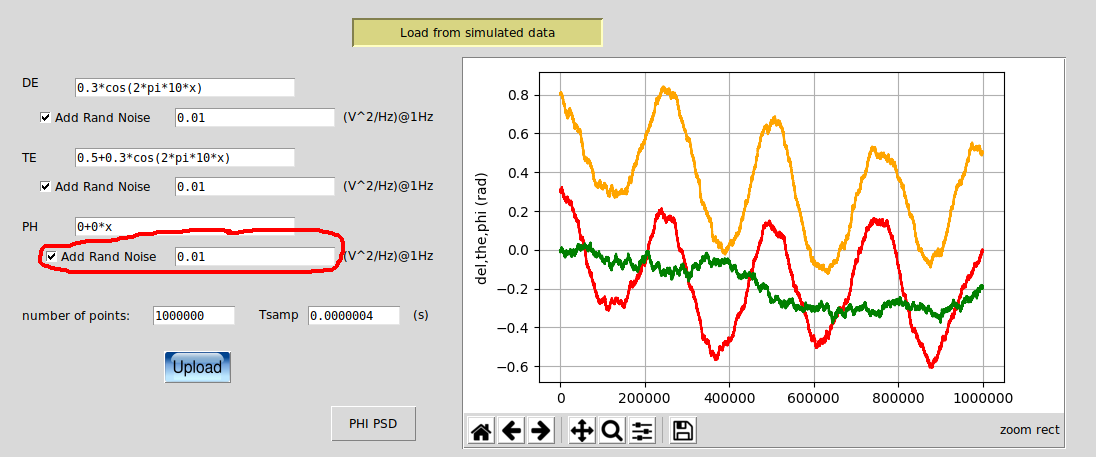
\includegraphics[width=1.15\textwidth]{immagini_noise/randwalk_par.png}}%
\caption{Optical fiber parameters ($\delta$,$\theta$) and metrological phase ($\phi$) chosen for the building of a simulated data set. Red circle shows the application of additional random walk noise}
\label{randwalk_par}
\end{figure}
\end{center}

\begin{figure}[hbtp]
\centering
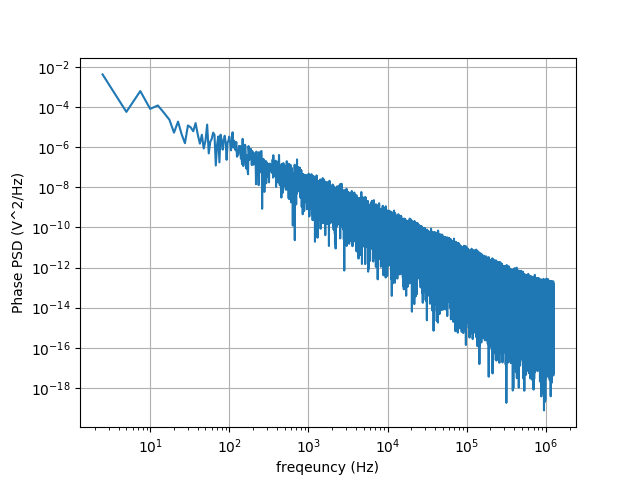
\includegraphics[scale=0.8]{immagini_noise/PSD_phi.png}
\caption{Phase PSD of the simulated data for $\phi$: $b_2$ (i.e. PSD @ 1Hz) corresponds to the chosen value in Fig.(\ref{randwalk_par}). (In this case, the value must be extrapolated due to the low resolution of the psd calculation. A resolution of 1Hz would require 2500000 data for a $F_s$=2500000 Hz)}
\label{PSD_phi}
\end{figure}

\clearpage

\subsection{Step 2: Electronic Noise on the DPOH channels}

At this step, the simulator produces the four lists of the Optical Hybrid channels (Fig.\ref{channels}). We then add to the channels respectively four independent white noise, following the assumed criterion $\frac{b_2}{b_0} \approx 10^{8}$ obtaining the data set shown in Fig.(\ref{channels_noise}). The corresponding four PSD spectra  are shown in Fig.(\ref{channels_noise}): due to the calculation involved in the the simulation (which represents the optical signal traveling in the fiber affected by birefringence) we see more peaks appear (e.g. at 20 Hz and 30 Hz). The  four spectra differ from each other because a particular incoming state of polarization has been fixed.

\begin{center}
\begin{figure}[hbtp]
 \makebox[\textwidth][c]{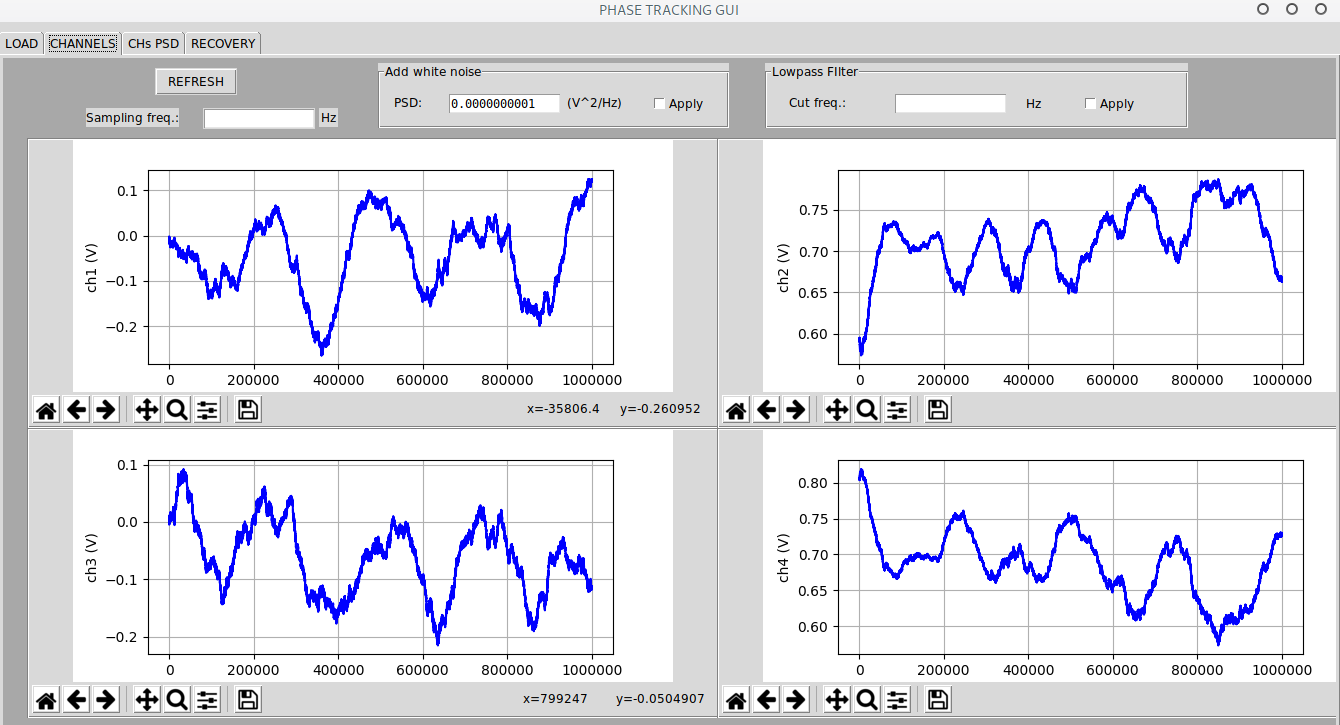
\includegraphics[width=1.1\textwidth]{immagini_noise/channels.png}}%
\caption{DPOH channels for set of simulated data.}
\label{channels}
\end{figure}
\end{center}

\begin{center}
\begin{figure}[hbtp]
 \makebox[\textwidth][c]{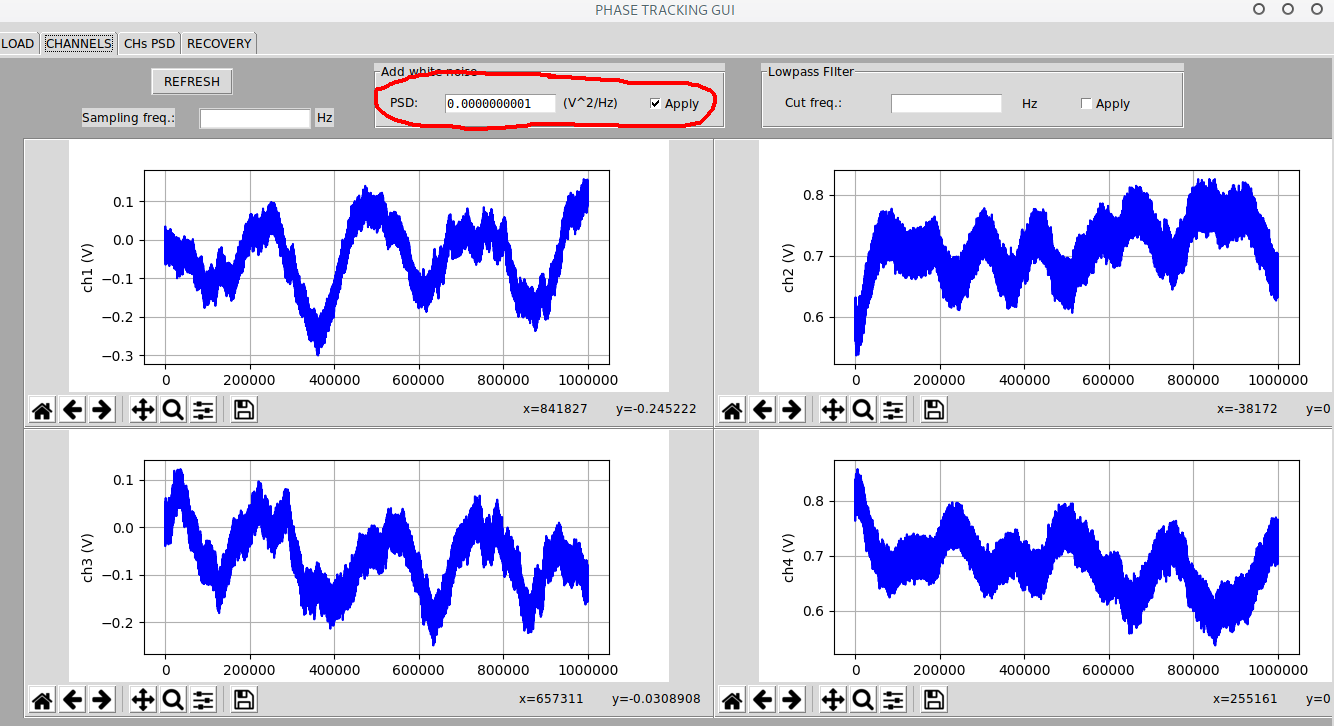
\includegraphics[width=1.1\textwidth]{immagini_noise/channels_noise.png}}%
\caption{DPOH channels for set of simulated data + white noise $10^{-9}$ \SI{}{\radian\squared\per\hertz}.}
\label{channels_noise}
\end{figure}
\end{center}


\begin{figure}[hbtp]
\centering
 \makebox[\textwidth][c]{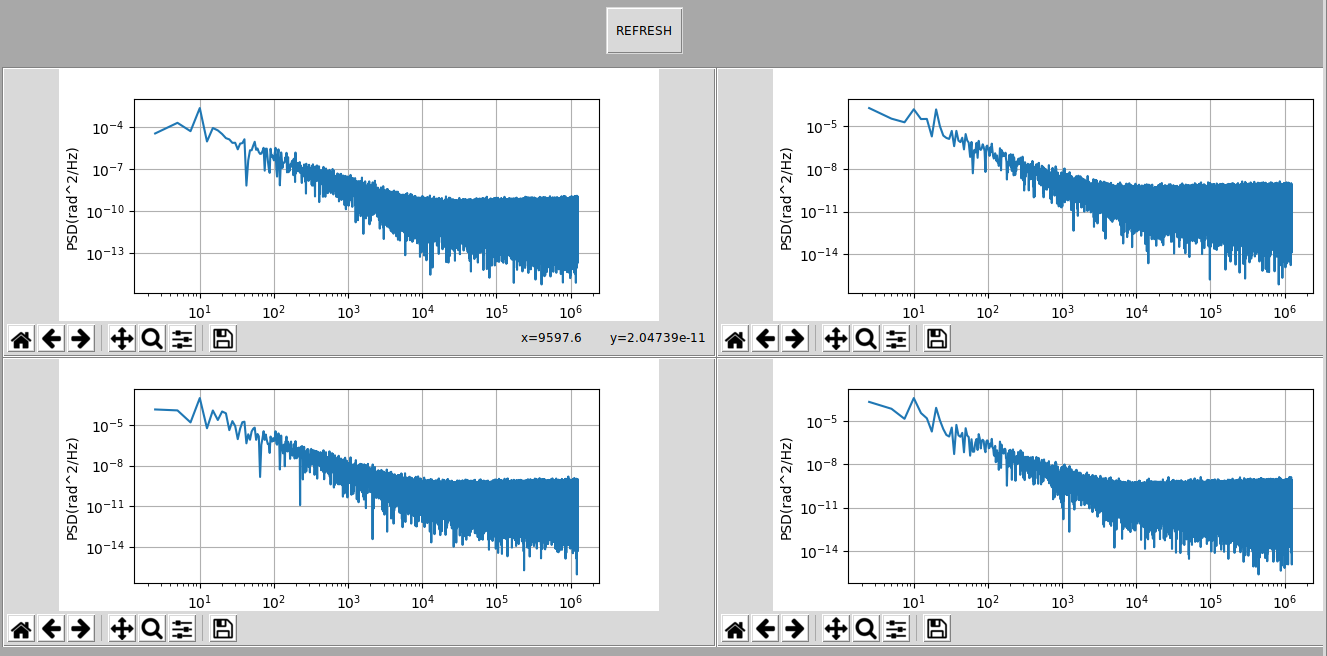
\includegraphics[width=1.1\textwidth]{immagini_noise/channels_psd.png}}%
\caption{PSD plots of the simulated channels (with the additional noise of Fig.{\ref{channels_noise}})}
\label{channels_psd}
\end{figure}



\pagebreak
\subsection{Step 3: Parameters recovery via LMS algorithm}
This section analyses the recovery algorithm response to the random walk and white noise intensities variations (Tab(\ref{pow-amp})). \\

First of all, the DSP structure of the algorithm in now simplified compared to the initial one and it is shown in Fig(\ref{scheme}) where the only check applied regards the periodicity of $\theta$ which is the more "unstable" parameter.\\

As an initial step, we neglect the additional white noise ($A_{\text{wn}}=0$) and we increase $A_{\text{rw}}$. The result for  $b_2=0.01$ \SI{}{\radian\squared\per\hertz}, which is a reasonable value as stated in Sec({\ref{back}}), is contained in Fig(\ref{recovery_Noise0_Rand-2}). As expected, the algorithm works properly with this level of noise: the residual phase is close to zero and the PSD spectrum reproduces the original one (compare Fig.(\ref{PSD_phi})). In the proximity of the singularity points, $\theta$ can experience jumps  which do not anyway affect the smoothness of $\phi$.\\
$A_{\text{rw}}$ has been raised to a level of even $b_2=1$ \SI{}{(\radian\squared\per\hertz)} and the recovery is still possible as as shown in Fig(\ref{recovery_Noise0_Rand1}). It should be noted that this last case is quite exaggerated and it is analyzed only for testing reasons, in fact phase variations around some radians per second (1000000 samples $\approx \frac{1}{2}$  s at 2500000 Hz sampling) do not represent often the reality.
\\

Thus, the next analysis focuses on the white noise simulation.\\
As a starting point value, we fix $b_0=10^{-10}$ as explained in Sec({\ref{back}}). Considering Fig.(\ref{white_par}) it can be seen that the recovery algorithm perform properly: in spite of the "jumping" trend experienced by the $\theta$ parameter, the metrological phase is tracked (with a residual following a white noise distribution with a variance compatible with $A_{\text{wn}}$ ). It should be observed again, that the "unstable" behaviour of theta occurs only near the singularities, as above. \\
The spontaneous test to do is now to increase the value of $b_0$ (namely the corresponding amplitude $A_{\text{wn}}$ of the disturbing signal ).
The recovery algorithm shows the ability to work for every value of noise \\ \underline{respecting a reasonable SNR ratio}: the ultimate supportable value for the data set considered in this example is up to $b_0=10^{-7}$. An example of failure is instead shown in Fig(\ref{failure}), where with $b_0=10^{-6}$, the plateau of the white noise reaches the peaks in the low frequency range which contains the useful information (see the input data in Fig.(\ref{recovery_Noise0_Rand-2})).


\pagebreak

\begin{figure}[hbtp]
\centering
 \makebox[\textwidth][c]{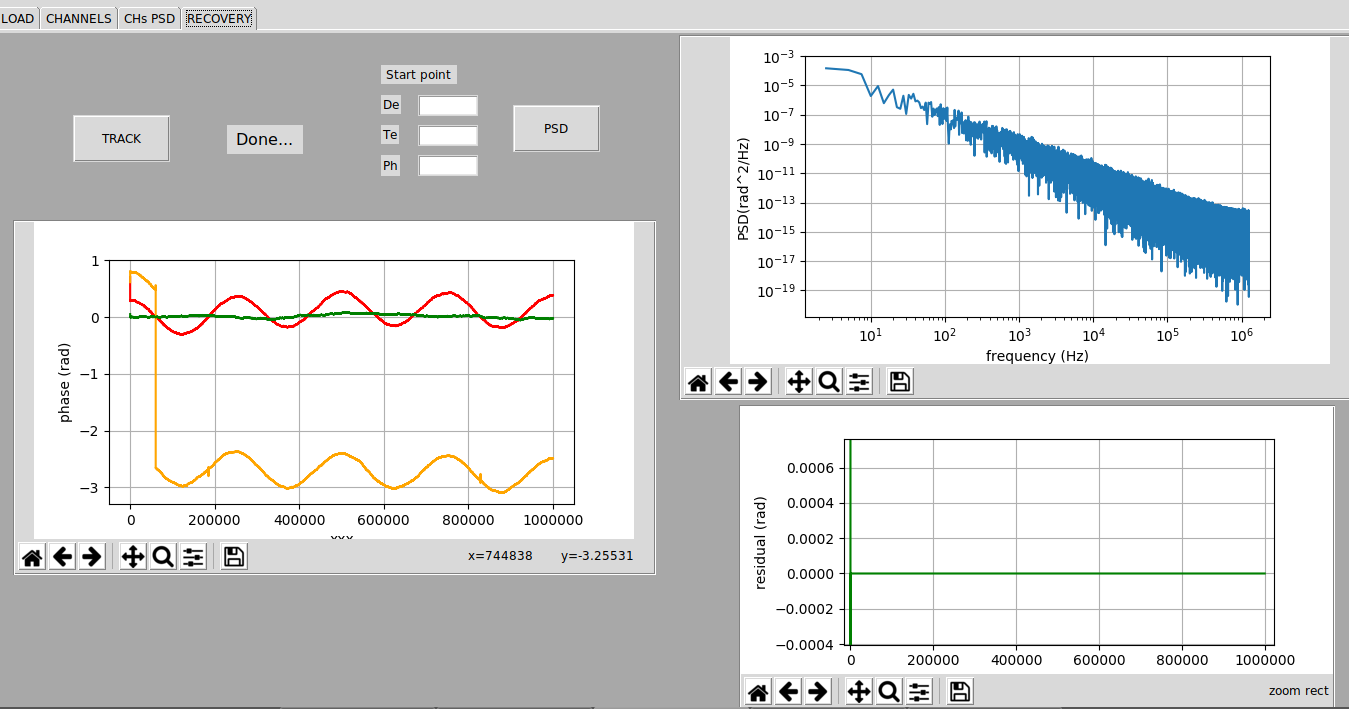
\includegraphics[width=0.97\textwidth]{immagini_noise/recovery_Noise0_Rand-2.png}}%
\caption{Recoverd parameters for $A_{\text{rw}}=0.01$ \SI{}{\radian\squared\per\hertz}, $A_{\text{wn}}=0$ \SI{}{\radian\squared\per\hertz}}
\label{recovery_Noise0_Rand-2}
\end{figure}

\begin{figure}[hbtp]
\centering
 \makebox[\textwidth][c]{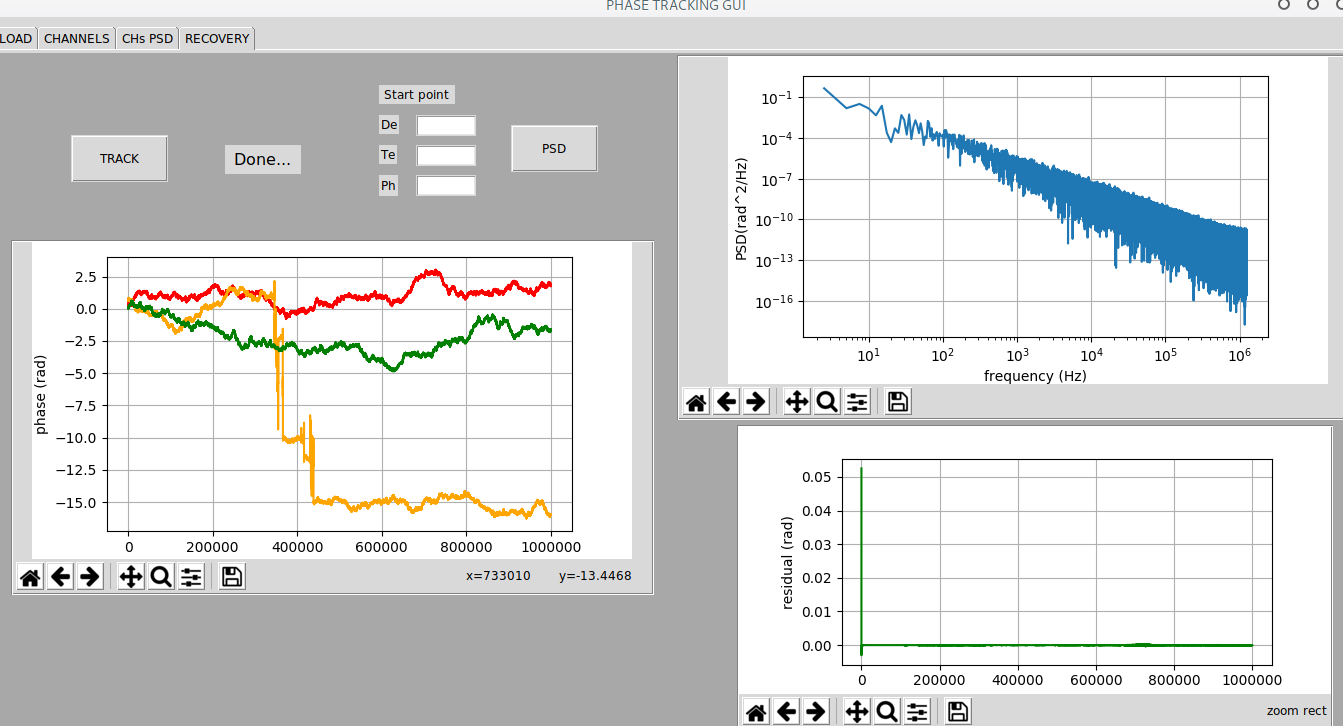
\includegraphics[width=0.97\textwidth]{immagini_noise/recovery_Noise0_Rand1.png}}%
\caption{Recoverd parameters for $A_{\text{rw}}=1$ \SI{}{\radian\squared\per\hertz}, $A_{\text{wn}}=0$ \SI{}{\radian\squared\per\hertz}}
\label{recovery_Noise0_Rand1}
\end{figure}

\begin{figure}[hbtp]
\centering
 \makebox[\textwidth][c]{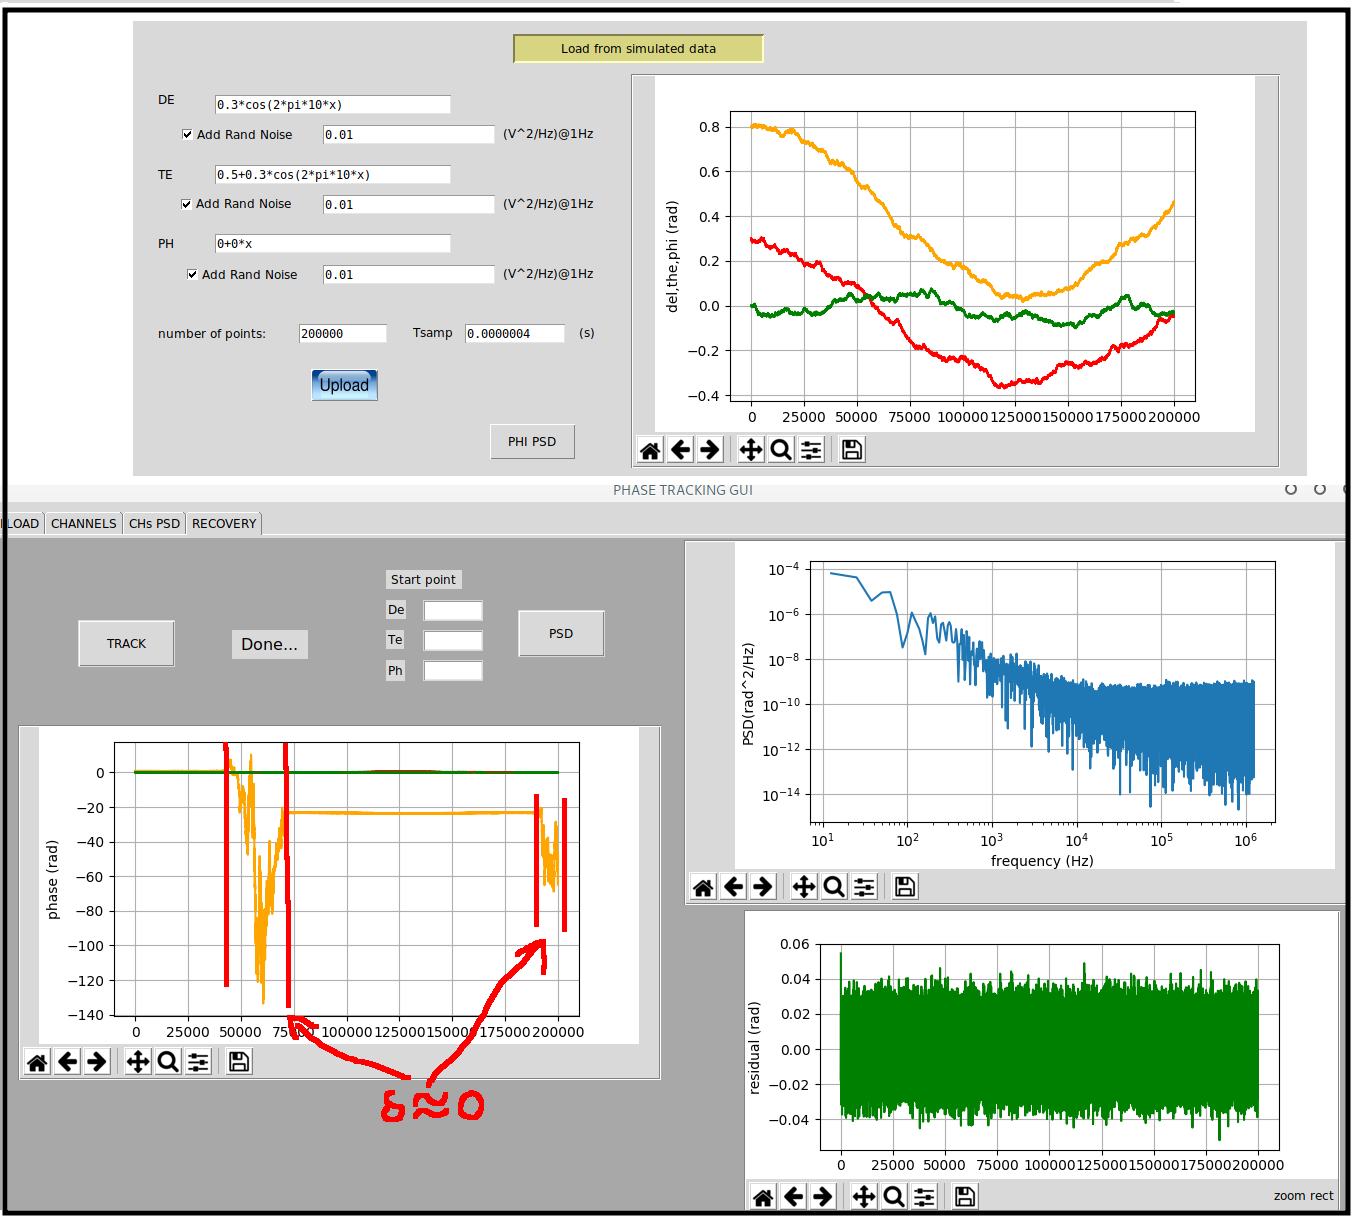
\includegraphics[width=1.1\textwidth]{immagini_noise/white_par.png}}%
\caption{Top: parameters data adopted in this notes for the white noise analysis. Bottom: recovered data for $b_0=10^{-10}$}
\label{white_par}
\end{figure}

\begin{figure}[hbtp]
\centering
 \makebox[\textwidth][c]{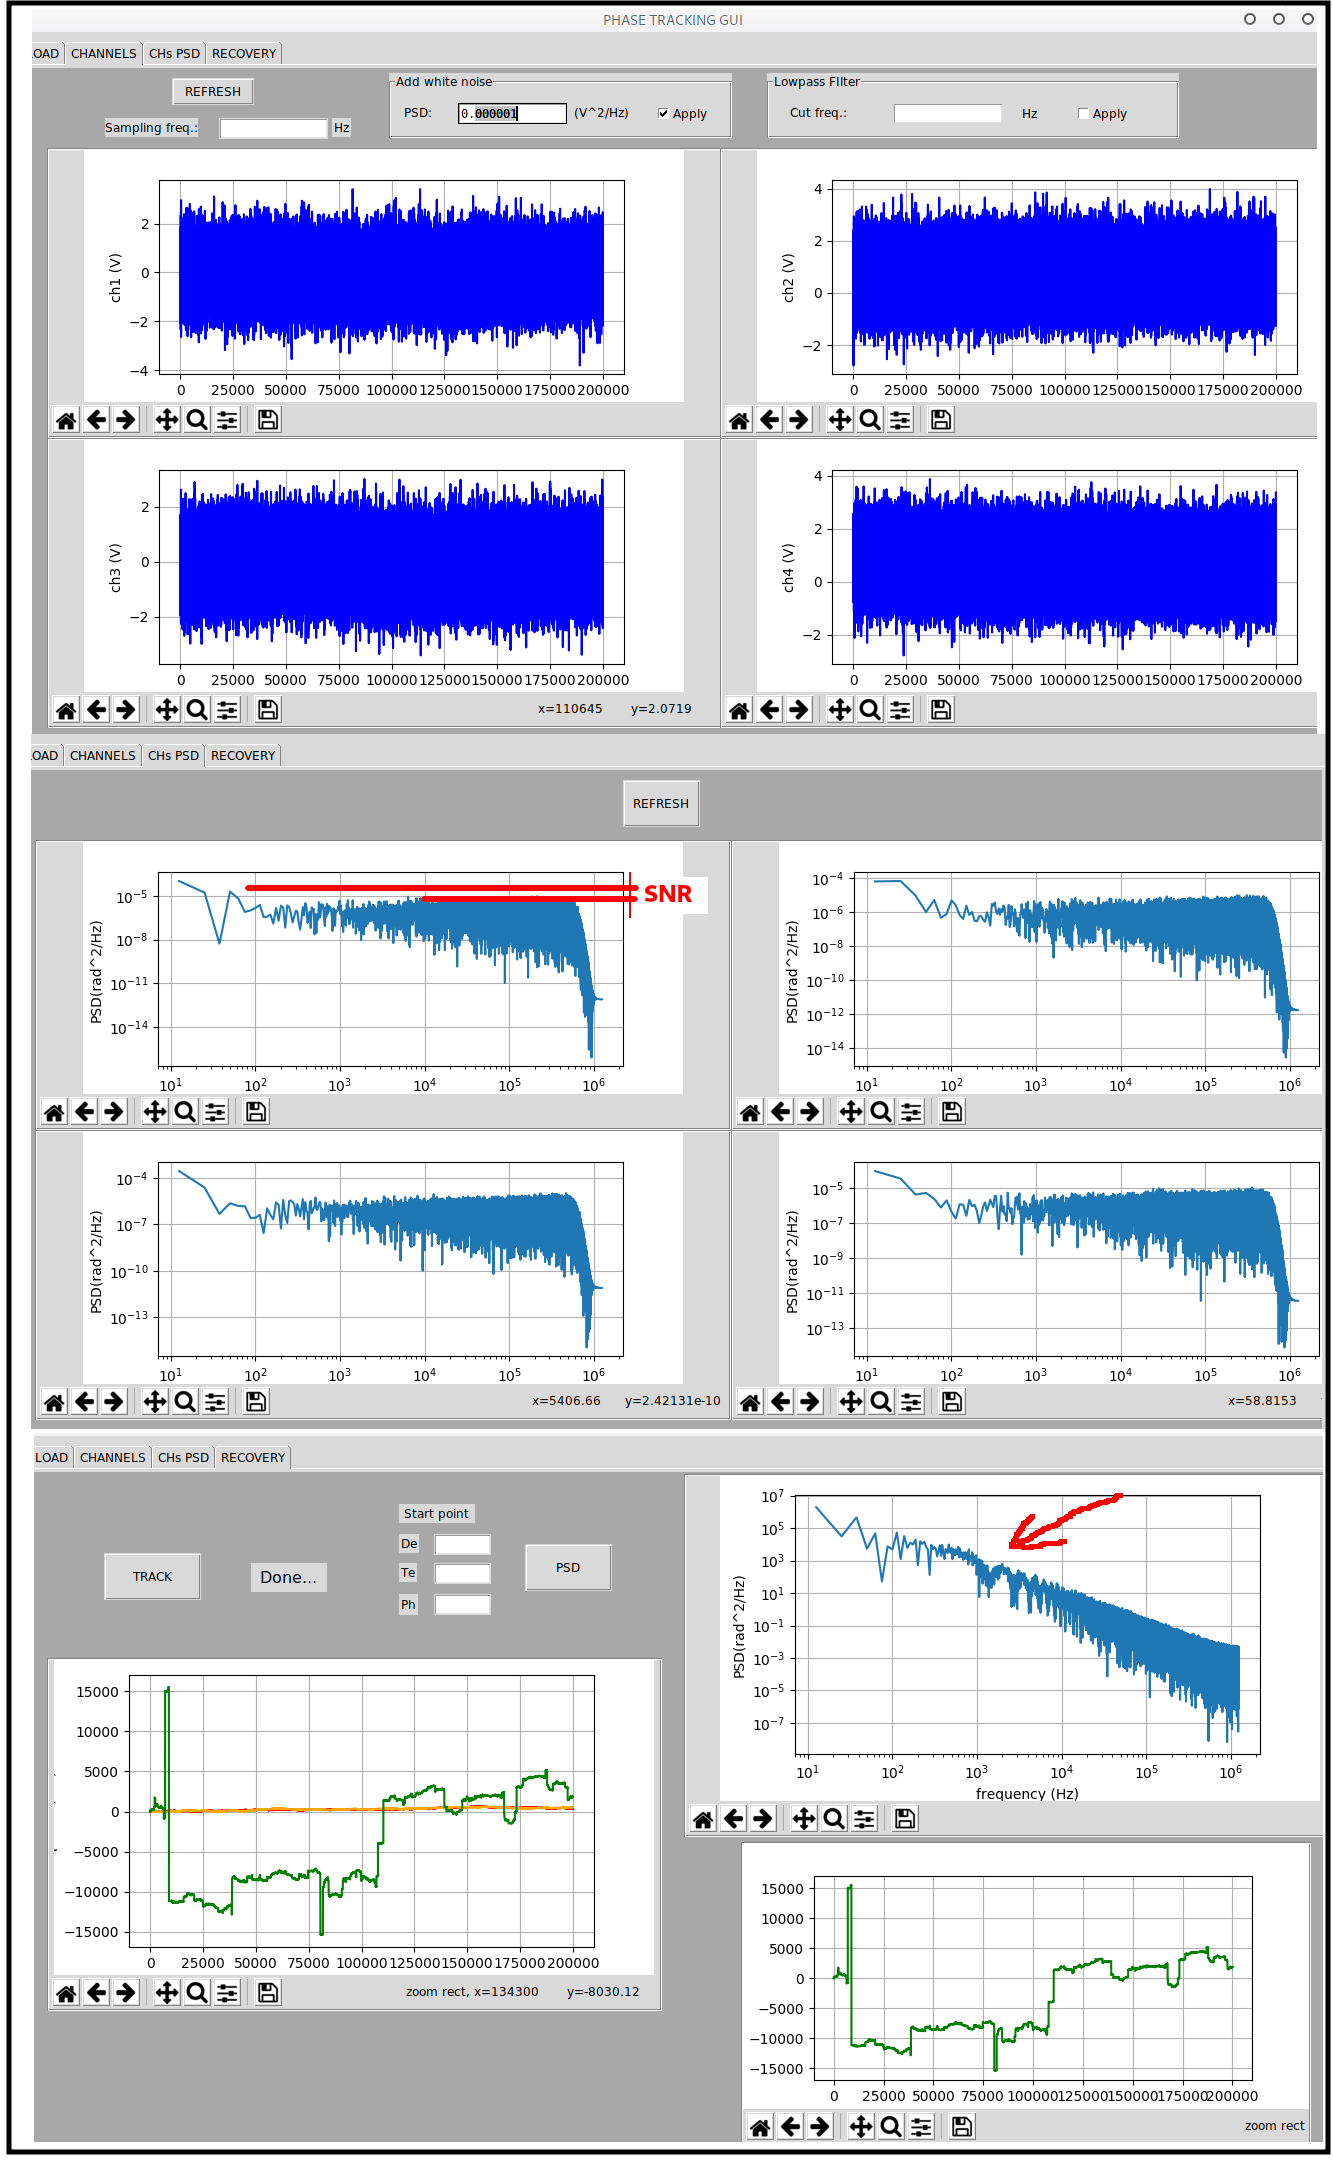
\includegraphics[width=0.95\textwidth]{immagini_noise/failure.png}}%
\caption{Failure of the recovery process for a too high value of white noise $b_0$}
\label{failure}
\end{figure}

\begin{figure}[hbtp]
\centering
 \makebox[\textwidth][c]{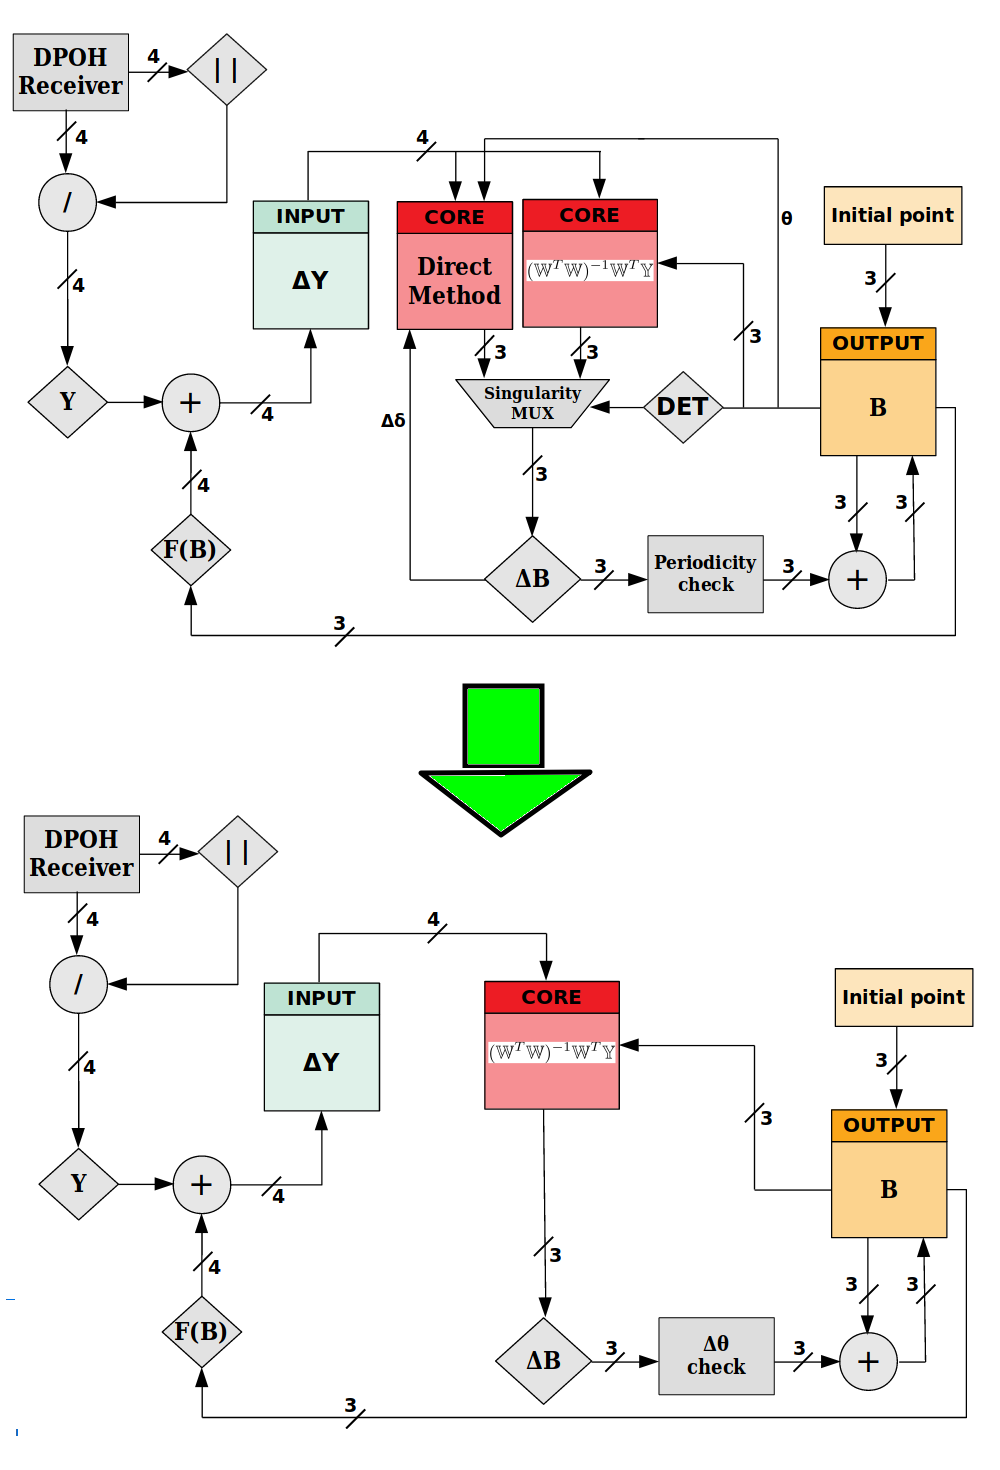
\includegraphics[width=0.95\textwidth]{immagini_noise/scheme.png}}%
\caption{Simplifications introduced in the algorithm}
\label{scheme}
\end{figure}

\end{document}
